
%(BEGIN_QUESTION)
% Copyright 2011, Tony R. Kuphaldt, released under the Creative Commons Attribution License (v 1.0)
% This means you may do almost anything with this work of mine, so long as you give me proper credit

This level-control system is supposed to maintain a constant liquid level inside the knockout drum, preventing liquid from entering the compressor as well as gas from entering the scavenging pump.  Yet, for some reason gas did manage to enter the scavenging pump, causing a major fire in that area leading to a complete shut-down of the unit:

$$\includegraphics[width=15.5cm]{i03411x01.eps}$$

A trend recording of liquid level and control valve position captured before the explosion holds the only clue as to why this happened.  Examine it to see if you can determine the source of the trouble:

$$\includegraphics[width=15.5cm]{i03411x02.eps}$$

\vfil 

\underbar{file i03411}
\eject
%(END_QUESTION)





%(BEGIN_ANSWER)

This is a graded question -- no answers or hints given!

%(END_ANSWER)





%(BEGIN_NOTES)

The trend holds all the clues for us here.  Here we see the level transmitter failed with a signal value ``frozen'' slightly above setpoint, causing the control valve position to integrate upward as indicated by the ramping output trend.  As the valve opened up wider and wider, the knockout drum level accelerated downward, letting all the liquid out of the drum and allowing gas to reach the scavenging pump.  In the immortal words of Beavis: {\it ``Fire!  Fire!  Fire!''}

\vskip 10pt

A general diagnostic tip for process troubleshooting is to remember that ``noise'' is a normal thing to see in a process variable trend.  If a trend goes from (normally) noisy to flat-line, something has most likely gone wrong with the sensing of that variable.  In fact, some smart pressure transmitter manufacturers equip their pressure sensors with a ``plugged line'' diagnostic to detect the plugging of impulse lines between the sensor and the process vessel, based on the amount of pressure ``noise'' seen by the transmitter over time.  If the transmitter's self-diagnostic algorithms detect substantially less pressure noise than normal, it flags an alarm calling for maintenance personnel to check the impulse line(s) for plugging.

%INDEX% Process troubleshooting: diagnosing problem via trend recording

%(END_NOTES)


